\section{Undirected Graphical Models}
A graph consists of a set of vertices (nodes), along with a set of edges joining some pairs of the vertices. In graphical models, each vertex represents a random variable, and the graph gives a visual way of understanding the joint distribution of the entire set of random variables. They can be useful for either unsupervised or supervised learning. In an undirected graph, the edges have no directional arrows. In undirected graphical models, also known as Markov random fields or Markov networks, the absence of an edge between two vertices has a special meaning: the corresponding random variables are conditionally independent, given the other variables.

The main challenges in working with graphical models are model selection (choosing the structure of the graph), estimation of the edge parameters from data, and computation of marginal vertex probabilities and expectations, from their joint distribution. The last two tasks are sometimes called learning and inference in the computer science literature.

There is a large and active literature on directed graphical models or Bayesian networks; these are graphical models in which the edges have directional arrows (but no directed cycles). Directed graphical models represent probability distributions that can be factored into products of conditional distributions, and have the potential for causal interpretations.

 A graph $G$ consists of a pair $(V, E)$, where $V$ is a set of vertices and $E$ the set of edges (defined by pairs of vertices). Two vertices $X$ and $Y$ are called adjacent if there is a edge joining them; this is denoted by $X \approx Y$. A path $X_1,X_2,\cdots,X_n$ is a set of vertices that are joined, that is $X_{i-1} \approx X_i$ for$ i = 2,\cdots,n$. A complete graph is a graph with every pair of vertices joined by an edge. A subgraph $U \in V$ is a subset of vertices together with their edges.
In a Markov graph $G$, the absence of an edge implies that the corresponding random variables are conditionally independent given the variables at the other vertices. This is expressed with the following notation:

\begin{equation}
\textit{No edge joining $X$ and $Y$} \Longleftrightarrow  X \perp Y|rest
\end{equation}
where \textit{rest} refers to the other vertices in the graph (first figure in \autoref{graphs}). These are known as \textit{pairwise Markov independencies} of $G$.

If $A$, $B$ and $C$ are subgraphs, then $C$ is said to separate $A$ and $B$ if every path between $A$ and $B$ intersects a node in $C$. For example, $Y$ separates $X$ and $Z$ in \autoref{graphs}(a) and \autoref{graphs}(d), and $Z$ separates $Y$ and $W$ in \autoref{graphs}(d). In '\autoref{graphs}(b) $Z$ is not connected to $X$,$Y$,$W$ so we say that the two sets are separated by the empty set. In \autoref{graphs}(c), $C = \{X,Z\}$ separates $Y$ and $W$.

Separators have the nice property that they break the graph into conditionally independent pieces. Specifically, in a Markov graph G with sub-graphs A, B and C,
\begin{equation}
\textit{if $C$ separates $A$ and $B$} \Rightarrow A\perp B|C
\end{equation}
These are known as the \textbf{global Markov properties} of $G$.

The global Markov property allows us to decompose graphs into smaller more manageable pieces and thus leads to essential simplifications in computation and interpretation. For this purpose we separate the graph into cliques. A \textbf{clique} is a complete subgraph a set of vertices that are all adjacent to one another; it is called \textbf{maximal}, if it is a clique and no other vertices can be added to it and still yield a clique. The maximal cliques for the graphs of \autoref{graphs} are
\begin{itemize}
\item $\{X, Y\}$, $\{Y, Z\}$;
\item $\{X, Y, W\}$, $\{Z\}$;
\item $\{X, Y\}$, $\{Y, Z\}, \{Z, W\},\{X, W\}$;
\item $\{X, Y\}$, $\{Y, Z\}, \{X, W\}$.
\end{itemize}

\begin{figure}
\centering
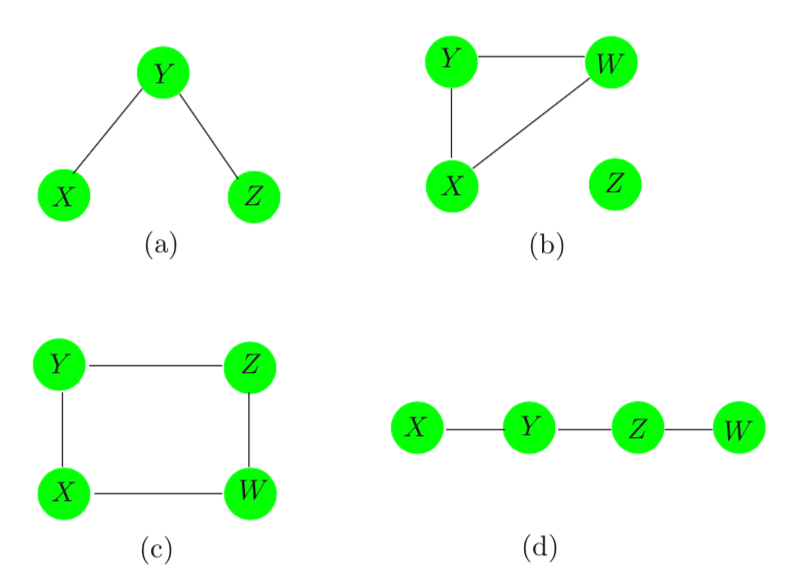
\includegraphics[scale=0.45]{img/graphs}
\caption{Examples of undirected graphical models or Markov networks. Each node or vertex represents a random variable, and the lack of an edge between two nodes indicates conditional independence. For example, in graph (a), $X$ and $Z$ are conditionally independent, given $Y$. In graph (b), $Z$ is independent of each of $X$, $Y$, and $W$.}
\label{graphs}
\end{figure}
A probability density function f over a Markov graph G can be can represented as
\begin{equation}
(x) = \frac{1}{Z} \prod_{C \in \CMcal{C}} \Psi_C (x_C)
\end{equation}
where $C$ is the set of maximal cliques, and the positive functions $\Psi C()$ are called clique potentials.  These are not in general density functions, but rather are affinities that capture the dependence in $X_C$ by scoring certain instances $X_C$ higher than others. The quantity
\begin{equation}
X = \sum_{x \in \CMcal{X}} \prod_{c \in \CMcal{C}} \X_C{x_C}
\end{equation}
is the normalizing constant, also known as the partition function

....
